\chapter{Forbidden histories}\label{ch:duality}

The preceding chapters described the \emph{admissible} histories. A rule is, however, naturally specified by what it \emph{forbids}, and the forbidden histories form a complex of their own. By Alexander duality its topology is that of the admissible complex, shifted by one dimension. For rules in which admissibility is decided by prefix sets, a class that contains every arithmetic rule of the Substrate (\cref{lem:F}), the forbidden complex collapses up to homotopy to a small combinatorial complex built from the prefix sets that can never be completed. The question ``is there a two-dimensional hole in $K_A$?'' becomes ``is there a one-dimensional cycle that does not bound in a complex on at most $62$ vertices?''. Homology has coefficients in $\F$, $k=6$ unless stated, and all complexes are finite. Alexander duality, the nerve theorem and Quillen's closure lemma are classical and are used as such.

\section{Flags, prefix sets and two dual spheres}\label{sec:flags}
Let $[k]=\{0,\dots,k-1\}$ and $\Pm$ the set of proper nonempty subsets of $[k]$. A \emph{flag} is a maximal chain $I_1\subset\dots\subset I_{k-1}$ in $\Pm$. Flags correspond bijectively to orderings $(x_1,\dots,x_k)$ of $[k]$ via $I_t=\{x_1,\dots,x_t\}$; $I_t$ is the $t$-th prefix set. Let $T=\Delta(\Pm)$ be the order complex of $\Pm$: its simplices are chains, it is the barycentric subdivision of the boundary of a $(k{-}1)$-simplex, hence a triangulated sphere $S^{k-2}$, and its facets are the flags.

The permutohedron $P_k$ has vertices indexed by orderings and proper faces $F(\pi)$ indexed by ordered partitions $\pi=(B_1|\dots|B_m)$ with $m\ge2$ blocks (\cref{def:faces}). To $\pi$ attach the chain
\[
c(\pi)=\{B_1,\ B_1\cup B_2,\ \dots,\ B_1\cup\dots\cup B_{m-1}\}\in T .
\]
This is a bijection between proper faces of $P_k$ and simplices of $T$; $F(\pi)\subseteq F(\pi')$ iff $c(\pi)\supseteq c(\pi')$; and a flag $f$ is a vertex of $F(\pi)$ iff $c(\pi)\subseteq f$. So $\partial P_k$ and $T$ are dual cell structures on the same sphere (\cref{fig:duality}).
\begin{definition}[forbidden complex]\label[definition]{def:forbidden}
For a set $A$ of orderings let $K_A\subseteq\partial P_k$ be the subcomplex of faces all of whose vertices lie in $A$ (\cref{def:KA}) and let the \emph{forbidden complex} $Y_A\subseteq T$ be the subcomplex generated by the flags of the orderings \emph{not} in $A$.
\end{definition}
\begin{proposition}[dictionary]\label[proposition]{prop:dict}
$F(\pi)\in K_A$ if and only if $c(\pi)\notin Y_A$.
\end{proposition}
\begin{proof}
$F(\pi)\in K_A$ iff every flag containing $c(\pi)$ is admissible, iff no non-admissible flag contains $c(\pi)$, iff $c(\pi)$ is not a face of a generator of $Y_A$.
\end{proof}

\begin{figure}[ht]\centering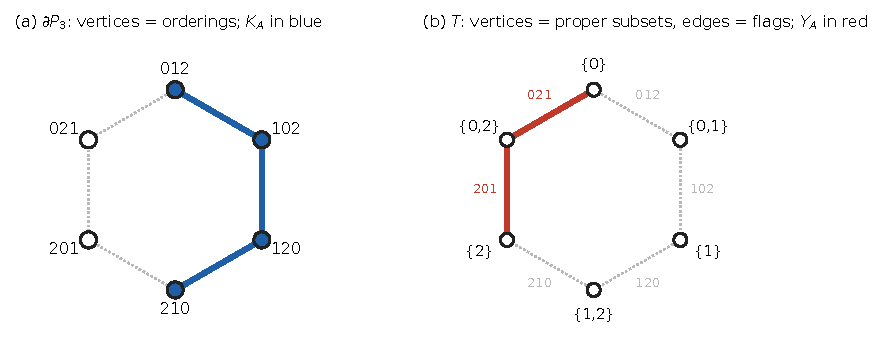
\includegraphics[width=\textwidth]{figures/fig_duality.pdf}
\caption{Duality for $k=3$, where everything can be seen. Left: the hexagon $\partial P_3$ with vertices the six orderings; $A$ consists of four consecutive orderings, and $K_A$ (blue) is the path they span. Right: the dual hexagon $T$, whose vertices are the six proper subsets and whose edges are the flags; $Y_A$ (red) is the subcomplex generated by the two flags of orderings not in $A$. The dictionary of \cref{prop:dict} matches each face of $K_A$ with a simplex of $T$ \emph{outside} $Y_A$. Here $\Hh_0(K_A)=0$ and $\Hh^{0}(Y_A)=0$ because $Y_A$ is connected (the two missing flags share the vertex $\{0,2\}$). Had the two missing orderings been non-adjacent, $K_A$ would have two components and $Y_A$ would be two disjoint edges, so both sides would be one-dimensional.}\label{fig:duality}
\end{figure}

\section{Alexander duality for history complexes}
\begin{theorem}[forbidden-history duality; analytic]\label[theorem]{thm:AD}
Let $\emptyset\ne A\subsetneq S_k$. For all $j$,
\[
\Hh_j(K_A;\F)\ \cong\ \Hh^{\,k-3-j}(Y_A;\F).
\]
In particular for $k=6$: $\beta_2(K_A)=\dim H_1(Y_A;\F)$, $\beta_1(K_A)=\dim\Hh_2(Y_A;\F)$, $\beta_3(K_A)=(\text{number of components of }Y_A)-1$, and $\beta_4(K_A)=0$.

\end{theorem}
\begin{proof}
\emph{Step 1: $|K_A|$ is a deformation retract of $S^{k-2}\setminus|Y_A|$.} Let $\operatorname{sd}T$ be the barycentric subdivision of $T$, the order complex of the poset $\mathcal S$ of simplices of $T$ under inclusion. The subcomplex $\operatorname{sd}Y_A$ is a full subcomplex of $\operatorname{sd}T$, so the standard lemma on complements of full subcomplexes (\cite[\S70]{Munkres}) shows that $|T|\setminus|Y_A|$ deformation retracts onto the full subcomplex $L$ of $\operatorname{sd}T$ spanned by the vertices not in $\operatorname{sd}Y_A$, i.e.\ by the simplices $c\in\mathcal S$ with $c\notin Y_A$. On the other hand $\operatorname{sd}(\partial P_k)$ is the order complex of the face poset of $\partial P_k$, and by the dictionary $\pi\mapsto c(\pi)$ this poset is anti-isomorphic to $\mathcal S$ (inclusion of faces corresponds to reverse inclusion of chains); an order complex is unchanged by reversing the order. So $\operatorname{sd}(\partial P_k)\cong\operatorname{sd}T$ compatibly with the identification of the sphere. By \cref{prop:dict} the cells of $K_A$ correspond exactly to the vertices of $L$, and $K_A$ is closed under faces (if $c\notin Y_A$ and $c'\supseteq c$ then $c'\notin Y_A$, since $Y_A$ is closed under subchains). Hence $L=\operatorname{sd}K_A$.
\emph{Step 2.} $Y_A$ is a nonempty proper subcomplex of the sphere $S^{k-2}$ ($A$ is proper and nonempty), compact and locally contractible, so Alexander duality (\cite[Thm.~3.44]{Hatcher}) gives $\Hh_j(S^{k-2}\setminus|Y_A|)\cong\Hh^{k-3-j}(Y_A)$ over $\Z$, hence over $\F$ by the universal coefficient theorem (all groups are finitely generated). Combine with Step~1. For $k=6$ the sphere is $S^4$; the Betti identities follow from $\dim\Hh^i=\dim\Hh_i$ over a field and $\dim\Hh^0(Y)=\#\mathrm{components}-1$.
\end{proof}
The theorem is why the whole programme can be phrased in terms of forbidden data: \emph{the topology of the history complex is the topology of the forbidden complex}. It explains where $\beta_2$ comes from; the nerve explains how to compute it cheaply.

\section{Dead sets and the nerve theorem}\label{sec:nerve}
\begin{definition}[prefix-defined, dead sets, dead-set nerve]\label[definition]{def:dead}
A system is \emph{prefix-defined} if there is a family $\mathcal A\subseteq\Pm$ such that an ordering is admissible iff all its prefix sets belong to $\mathcal A$ (\cref{def:prefix-defined}). A set $I\in\Pm$ is \emph{dead} if every flag through $I$ is non-admissible; $D=D_A$ denotes the set of dead sets. For $\mathcal T\subseteq\Pm$ put
\[
Q_{\mathcal T}=\{x\in\Pm:\ x\text{ is comparable ($\subseteq$ or $\supseteq$) to every }t\in\mathcal T\}.
\]
The \emph{dead-set nerve} $N[D]$ is the simplicial complex on $D$ whose simplices are the nonempty $\mathcal T\subseteq D$ with $Q_{\mathcal T}\neq\emptyset$.
\end{definition}
Every $I\notin\mathcal A$ is dead, since $I$ is a prefix set of every flag through it, but a set in $\mathcal A$ can be dead too, if every way of completing it passes through a forbidden set. In $N[D]$ two dead sets are joined unless they are complementary, and three form a triangle iff some set is comparable to all of them.
\begin{lemma}[closure lemma; \cite{Quillen}]\label[lemma]{lem:quillen}
If $\varphi:Q\to Q$ is an order-preserving self-map of a finite poset with $\varphi(x)\ge x$ for all $x$ and $\varphi\circ\varphi=\varphi$, then $\Delta(Q)\simeq\Delta(\varphi(Q))$.

\end{lemma}
\begin{lemma}[star-intersection lemma; analytic]\label[lemma]{lem:star}
For every nonempty $\mathcal T\subseteq\Pm$ the set $Q_{\mathcal T}$ is empty or $\Delta(Q_{\mathcal T})$ is contractible.

\end{lemma}
\begin{proof}
Let $x_0\in Q_{\mathcal T}$.
\emph{Case 1: some $t\in\mathcal T$ satisfies $t\subseteq x_0$.} Put $a=\bigcup\{t\in\mathcal T:\ t\subseteq x_0\}$; then $\emptyset\neq a\subseteq x_0$, so $a\in\Pm$. Define $\varphi(x)=x\cup a$ on $Q_{\mathcal T}$. We check $\varphi(x)\in Q_{\mathcal T}$. Let $t\in\mathcal T$. If $t\subseteq x_0$ then $t\subseteq a\subseteq\varphi(x)$. Otherwise $x_0\subsetneq t$ (as $x_0$ is comparable to $t$), so $a\subseteq t$; if $x\subseteq t$ then $\varphi(x)\subseteq t$, and if $t\subseteq x$ then $t\subseteq\varphi(x)$. Next $\varphi(x)\ne[k]$: if $x\subseteq t$ for some $t\in\mathcal T$, then either $t\not\subseteq x_0$ and $\varphi(x)\subseteq t$, or $t\subseteq x_0$ and $x\subseteq t\subseteq a$, whence $\varphi(x)=a\subseteq x_0$; if $x\not\subseteq t$ for all $t$, then $t\subseteq x$ for all $t$, so $a\subseteq x$ and $\varphi(x)=x$. Thus $\varphi$ is a well-defined, order-preserving, extensive, idempotent map. Its image is $\{x\in Q_{\mathcal T}:\ x\supseteq a\}$, which has least element $a$ (indeed $a\in Q_{\mathcal T}$: $t\subseteq a$ for $t\subseteq x_0$, and $a\subseteq x_0\subsetneq t$ otherwise). A poset with a least element has a contractible order complex; apply \cref{lem:quillen}.
\emph{Case 2: no $t\in\mathcal T$ satisfies $t\subseteq x_0$.} Then $x_0\subsetneq t$ for all $t$, so $V=\bigcap\mathcal T\supseteq x_0$ is nonempty and proper. Define $\varphi(x)=x\cup V$. For $t\in\mathcal T$: $V\subseteq t$, so $x\subseteq t\Rightarrow\varphi(x)\subseteq t$ and $t\subseteq x\Rightarrow t\subseteq\varphi(x)$; and $\varphi(x)\ne[k]$ because either $x\subseteq t$ for some $t$ (then $\varphi(x)\subseteq t$) or $x\supseteq t$ for all $t$ (then $x\supseteq V$ and $\varphi(x)=x$). The image $\{x\in Q_{\mathcal T}:\ x\supseteq V\}$ has least element $V$; conclude as before.
\end{proof}
\begin{theorem}[dead-set nerve theorem; analytic]\label[theorem]{thm:nerve}
Let $A$ be prefix-defined with $\emptyset\ne A\subsetneq S_k$. Then $Y_A\simeq N[D_A]$. Consequently
\begin{gather*}
\Hh_j(K_A)\ \cong\ \Hh^{\,k-3-j}(N[D_A]),\\
\text{and for }k=6:\quad \beta_2(K_A)=\dim H_1(N[D_A];\F),\quad \beta_1(K_A)=\dim\Hh_2(N[D_A];\F).
\end{gather*}

\end{theorem}
\begin{proof}
For $I\in\Pm$ the closed star of the vertex $I$ in $T$ is $\operatorname{St}(I)=\Delta(Q_{\{I\}})$. We claim $Y_A=\bigcup_{I\in D}\operatorname{St}(I)$. A simplex of $\operatorname{St}(I)$ with $I$ dead is a chain $c$ with $c\cup\{I\}$ a chain, hence contained in a flag through $I$, which is non-admissible; so $c\in Y_A$. Conversely a generator of $Y_A$ is a non-admissible flag; by prefix-definedness it has a prefix set $I\notin\mathcal A$, which is dead, so the flag lies in $\operatorname{St}(I)$. For nonempty $\mathcal T\subseteq D$,
$\bigcap_{I\in\mathcal T}\operatorname{St}(I)=\Delta(\bigcap_IQ_{\{I\}})=\Delta(Q_{\mathcal T})$ (a chain lies in all stars iff all its members are comparable to every $I\in\mathcal T$). By \cref{lem:star} every nonempty intersection is contractible, so the nerve theorem for finite covers of a simplicial complex by subcomplexes gives $Y_A\simeq$ the nerve of $\{\operatorname{St}(I)\}_{I\in D}$, whose simplices are the $\mathcal T$ with $Q_{\mathcal T}\ne\emptyset$, i.e.\ $N[D]$. The Betti formulas follow from \cref{thm:AD}.
\end{proof}
\begin{corollary}[dead-set certificate]\label[corollary]{cor:dead-cert}
If $N[D_A]$ contains a $1$-cycle $z$ and an edge cocycle $c$ with $c(\partial\tau)=0$ for every triangle $\tau$ of $N[D_A]$ and $c(z)=1$, then $\beta_2(K_A)>0$. Conversely every system with $\beta_2(K_A)>0$ has such a pair.
\end{corollary}
\begin{proof}
$[z]\neq0$ in $H_1(N[D])$ by the argument of \cref{lem:certificate}; the converse is linear algebra over a field ($H^1\cong H_1^\ast$). Apply \cref{thm:nerve}.
\end{proof}
\begin{proposition}[arithmetic admissibility is prefix-defined]\label[proposition]{prop:arith-prefix}
For distinct positive integers $\ell_x$ ($x\in[k]$) and $m\ge1$, an ordering $(x_1,\dots,x_k)$ is SELECT-II admissible iff for every prefix set $I$ the number $m\prod_{x\in I}(\ell_x+1)^2/\ell_x$ is an integer. Hence arithmetic systems are prefix-defined with $\mathcal A=\{I:\ D(I)\mid m\}$.

\end{proposition}
\begin{proof}
See \cref{lem:F}: by induction $m_{t-1}=m\prod_{s<t}(\ell_{x_s}+1)^2/\ell_{x_s}$ is an integer as long as the earlier steps were admissible, and step $t$ is admissible iff $\ell_{x_t}\mid m_{t-1}$, which (as $\gcd(\ell+1,\ell)=1$) is equivalent to $m_{t-1}(\ell_{x_t}+1)^2/\ell_{x_t}\in\Z$.
\end{proof}

\section{The cycles that carry the holes}\label{sec:cycles}
For a regime the dead sets are computed directly. A triple of dead sets is \emph{hollow} if its three pairs are edges of $N[D]$ (no two complementary) but no set is comparable to all three. A hollow triangle is a $1$-cycle of $N[D]$; it is non-bounding iff it is not a sum of boundaries of triangles.
\begin{figure}[ht]\centering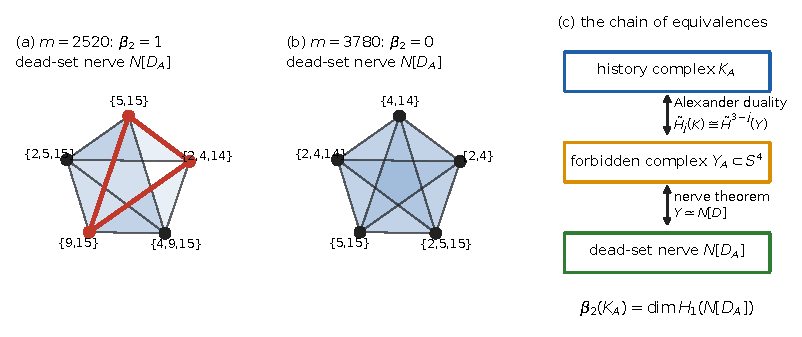
\includegraphics[width=\textwidth]{figures/fig_nerves.pdf}
\caption{Dead-set nerves, recomputed exactly. (a),(b)~Content $(2,4,5,9,14,15)$ at sources $2520$ and $3780$; both systems have $540$ admissible histories and five dead sets and differ in \emph{which} sets are dead. In (a) the red cycle is the hollow triangle $\{2,4,14\},\{5,15\},\{9,15\}$, which does not bound, so $\beta_2=1$; in (b) the nerve is contractible. (c)~The chain of equivalences $\beta_2(K_A)=\dim H_1(Y_A)=\dim H_1(N[D_A])$ (\cref{thm:AD,thm:nerve}).}\label{fig:nerves}
\end{figure}
\begin{proposition}[the sharp pair; finite-exact]\label[proposition]{prop:pair}
For content $(2,4,5,9,14,15)$ the system at source $2520$ has dead sets $\{2,4,14\},\{5,15\},\{2,5,15\},\{9,15\},\{4,9,15\}$ and $\beta_2=1$: the hollow triangle formed by $\{2,4,14\}$, $\{5,15\}$, $\{9,15\}$ is non-bounding and $H_1(N[D])\cong\F$. At source $3780$ the sets $\{9,15\},\{4,9,15\}$ are replaced by $\{2,4\},\{4,14\}$, the nerve is acyclic and $\beta_2=0$. Content $(2,3,4,5,8,15)$ with sources $480$ and $800$ has $|D|=11$ and $7$, $14$ non-bounding hollow triangles versus none, and $\beta_2=1$ versus $0$.

\end{proposition}
The pair at $2520/3780$ is the smallest exhibit: the two systems agree on $N$, $E$, $Q$, $h_1$, $h_q$, $S_B$ and $S_{d2}$ (\cref{ex:pair}) and differ in the radius-two data, but in forbidden-history terms they differ in \emph{which two dead sets} are present, and the nerve cycle is the mechanism.
\begin{observation}[census of the cycles; finite-exact]\label[observation]{obs:cycle-census}
Among the $290$ regimes with $\beta_2>0$ identified (the $158$ positives of the exhaustive census of $346{,}859$ six-label regimes and $132$ positives of a held-out sample of $263{,}124$), $288$ contain a non-bounding hollow triangle ($35$ types up to relabelling by $S_6$); each of the remaining two contains a non-bounding $4$-cycle $X,Y,Y\cup\{e\},X\cup\{e\}$ with $X\sqcup Y\sqcup\{e\}=[6]$, two \emph{complementary dead-set pairs} $\{X,Y\cup e\},\{Y,X\cup e\}$ (a ``complementary square'', the equator of a cross-polytope). Of $1000$ sampled regimes with $\beta_2=0$, $707$ contain hollow triangles, but \emph{none} contains a non-bounding one. All $290$ positives carry an explicit certificate $(z,c)$ in the sense of \cref{cor:dead-cert}.
The absence of a \emph{cone point} --- a dead set making all three pairs of a hollow triangle faces together with it, which trivially fills the triangle --- is \emph{not} equivalent to non-boundedness: $6$ hollow triangles among positives and $105$ among negatives have no cone point yet bound through longer fillings. A sharp purely local criterion for non-boundedness is not known.

\end{observation}
In the four census classes with equal $(N,h_1,Q,S_{ds})$ containing both signs, $S_{s2}$ of the positive system is smaller than that of the negative (differences $-16,-16,-16,-48$), and positives have dead sets of smaller size. This is an observation; no derivation of $S_{s2}$ from the nerve is known. Likewise the arithmetic thresholds produce dead sets that are pairwise compatible but have no common comparable set; that is a description of the examples, not an explanation.

\section{Certificates}\label{sec:certificates}
A stand-alone checker (about $200$ lines of Python, standard library only, importing nothing from the research code) recomputes dead sets from the arithmetic definition, builds $N[D]$, checks $\beta_2(K_A)=\dim H_1(N[D])$ from the definition of $K_A$ for four systems, and checks for each of the $290$ stored certificates that $c(\partial\tau)=0$ on every triangle and $c(z)=1$. All checks passed when it was run (\cref{app:status}). The check is sensitive: deleting one cocycle edge from one certificate, or replacing one certificate's cycle by another's, makes it report a failure. The check uses no elimination, only evaluation of the certificate.
